\section{Method}

\subsection{Network architecture}


\begin{figure}
\centering

% TODO should mention sizes! Maybe represent decoder output differently.

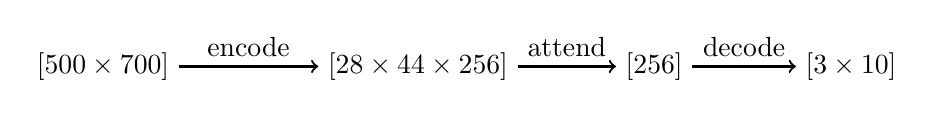
\begin{tikzpicture}
% 900, 1500, 1
% 28, 44, 256
% 1, 1, 256
% 3, 10

    \node (input) at (0,0) {$[500 \times 700]$};
    \node (encoded) at (4, 0) {$[28 \times 44 \times 256]$};
    \node (attended) at (7, 0) {$[256]$};
    \node (decoded) at (9.5, 0) {$[3 \times 10]$};

%   \pic [fill=cyan, draw=blue] at (-1,0) {annotated cuboid={width=1, height=900, depth=1500}};
%   \pic [fill=cyan, draw=blue] at (4,-0.5) {annotated cuboid={width=256, height=28, depth=44}};
%   \pic [fill=cyan, draw=blue] at (7,-0.5) {annotated cuboid={width=256, height=1, depth=1}};
%   \pic [fill=cyan, draw=blue] at (9,1.5) {annotated cuboid={width=1, height=10, depth=3}};

  \draw [->,thick] (input) -- node [above] {encode} (encoded);
  \draw [->,thick] (encoded) -- node [above] {attend} (attended);
  \draw [->,thick] (attended) -- node [above] {decode} (decoded);

\end{tikzpicture}

\caption{Overview of how the data flows in the proposed network. First the encoder produces a matrix of feature vectors, each corresponding to a different but overlapping location in the input image. Secondly, the attention aggregates the feature vectors into a single feature vector. Lastly, the decoder produces three softmax outputs, one for each digit.}
\label{fig:sys_overview}
\end{figure}


We now describe the different parts of the proposed network. See figure \ref{fig:sys_overview} for an overview of how the different parts of the network interact.

\subsubsection{Encoder}

\begin{figure}
\centering

\begin{tikzpicture}
% (1, 900, 1500, 1)
% (1, 450, 750, 4)
% (1, 225, 375, 16)
% (1, 225, 375, 32)
% (1, 112, 187, 32)
% (1, 112, 187, 128)
% (1, 56, 93, 128)
% (1, 56, 89, 256)
% (1, 28, 44, 256)

%   \pic {annotated cuboid};
  \pic [fill=cyan, draw=blue] at (0,0) {annotated cuboid={width=32, height=900, depth=1500}};
  \pic [fill=cyan, draw=blue] at (0.5,0) {annotated cuboid={width=32, height=900, depth=1500}};

  \pic [fill=yellow, draw=white] at (1.5,-0.5) {annotated cuboid={width=32, height=450, depth=750}};
  \pic [fill=cyan, draw=blue] at (2.1,-0.5) {annotated cuboid={width=64, height=450, depth=750}};
  \pic [fill=cyan, draw=blue] at (2.7,-0.5) {annotated cuboid={width=64, height=450, depth=750}};

  \pic [fill=yellow, draw=white] at (3.5,-0.7) {annotated cuboid={width=64, height=225, depth=375}};
  \pic [fill=cyan, draw=blue] at (4.5,-0.7) {annotated cuboid={width=128, height=225, depth=375}};

  \pic [fill=yellow, draw=white] at (5.5,-0.7) {annotated cuboid={width=128, height=112, depth=187}};
  \pic [fill=cyan, draw=blue] at (6.5,-0.7) {annotated cuboid={width=128, height=112, depth=187}};

  \pic [fill=yellow, draw=white] at (7.5,-0.8) {annotated cuboid={width=128, height=56, depth=93}};
  \pic [fill=green, draw=blue] at (9,-0.8) {annotated cuboid={width=256, height=56, depth=89}};

  \pic [fill=yellow, draw=white] at (10.5,-0.8) {annotated cuboid={width=256, height=28, depth=44}};

%   \pic [fill=magenta, text=blue, draw=blue] at (5,0) {annotated cuboid={width=2, height=50, depth=30}};
%   \pic [fill=green, text=green!50!black, draw=green!25!black] at (5,-2) {annotated cuboid={width=6, height=20, depth=15, units=mm}};
%   \pic at (1,-3) {annotated cuboid={width=150, height=200, depth=250, scale=.01, units=m}};
%   \pic [fill=cyan, text=blue!75!cyan, draw=blue!75!cyan] at (-3,-2) {annotated cuboid={width=15, height=18, depth=13.5, units=}};
\end{tikzpicture}

\caption{Proposed architecture for the encoder. Convolutional layers are blue (3x3) and green (1x5) while max pool layers are yellow (2x2).
The number below each layer indicate the depth of the layer.}
\label{fig:encoder}
\end{figure}


For encoder, we use a CNN with 7 convolutional layers with additional pooling layers, see figure \ref{fig:encoder}.
% We experimented with several different variations in number of convolution layers, pooling layers and layer depths before choosing this model.
Two consecutive 3x3 convolutional layers is a refactoring of a single 5x5 layer as suggested by \textcite{InceptionV3}. Thus, the first four convolutional layers correspond to two 5x5 convolutional layers with pooling, similar to the original single-digit CNN classifier \cite{lecun_1989} but with greater depth.

The number of pooling layers, number of convolutional layers and depth per layer were determined experimentally. The final encoder design, depicted in figure \ref{fig:encoder}, is somewhat similar to the encoder used in \cite{FornesCnnCategorization} except that we use more aggressive pooling. This is necessary because in our work, we input images of entire pages, while \textcite{FornesCnnCategorization} classify word images, which presumably are much smaller.

%The first four layers correspond closely to the original single digit classifier CNN \cite{lecun_1989} with the exception

% The number of layers and their depth was determined experimentally on the synthesized dataset using previous work as starting point \cite{FornesCnnCategorization}.



\subsubsection{Attention model}

Another major difference between our work and \cite{FornesCnnCategorization} is that although we both use variable input size, they use \textbf{Spatial pyramid pooling}, while we apply a soft attention model as presented in \cite{AttendAndTell}. As presented in section \ref{ssec:attention}, the encoder output can be seen as a list of feature vectors $\mathbf{a_i} \in \mathbb{R}^D$, which correspond to different, but overlapping, locations in the input image. The number of produced feature vectors depends on the size of the input image. We will see that this attention model aggregates all feature vectors $\mathbf{a_i}$ into a single fixed size vector $\mathbf{z} \in \mathbb{R}^D$.

The attention model consists of a multilayer perceptron, which for each feature vector $\mathbf{a_i}$ computes a salience score $e_i$:

\[
e_i = f_\text{att}(\mathbf{a_i})
\]

Note that this MLP does not have access to any information about the corresponding location of $\mathbf{a_i}$, thus the network must learn to recognize important parts by looking at the encoded features alone instead of learning to always look at a certain position in the input image. This is especially important for population records, where the relevant information can be in different locations depending on scribe and time period.

% We normalize the $e_i$ into $\alpha_i$ by computing the softmax.
% We normalize the $e_i$ by softmax and call the corresponding values attentions

We denote the softmax of $e_i$ as attentions $\alpha_i$, which sums to one by definition of softmax.
%We compute the softmax of $e_i$ as $\alpha_i$, which sums to one per definition.
We then use the attentions $\alpha_i$ as weights over the feature vectors:

\[
\mathbf{z} = \sum_{k=1}^L \alpha_i \mathbf{a_i}
\]

% Note that the spatial information about where in the image $\mathbf{z}$ comes from is lost in this sum.

%So just like the attention MLP, the decoder also becomes invariant to the object's position in the input image.

\subsubsection{Decoder}

The decoder employs an MLP for classifying the aggregated feature vector $\mathbf{z} \in \mathbb{R}^D$ from the attention model.
If $\mathbf{z}$ had a variable length, then we would need a different number of weights in the MLP for each different input size. Since the attention model produces a fixed size output independent of input size we avoid the problem of variable number of parameters.

Because $\mathbf{z}$ is summed over all locations, it does not contain any spatial information about where detected features come from.
Thus, the decoder is invariant to the location of detected objects, just like the attention model.

The proposed decoder MLP consists of an input layer of size $D$, one fully connected layer of $1024$ neurons with dropout and three parallel readout layers $D_1$, $D_2$ and $D_3$. Each of these three readout layers has a size of $10$ neurons and corresponds to a single digit in the range zero to nine.
Because the years we will extract are all in the range 1627--1890, $3$ digits is more than enough to classify year.

We do softmax on each readout layer to get pseudo-probabilities for the digits.
To compute the probability for a specific 3-digit sequence $\langle x, y, z \rangle$ we simply multiply the probability of each digit:

\[
P(D_1=x, D_2=y, D_3=z) = P(D_1=x) P(D_2=y) P(D_3=z)
\]


\subsection{Training procedure}
% TODO Perhaps make this a different section?

Here we describe how we train and evaluate the different models.

\subsubsection{Multi-year labels}

As presented in section \ref{sssec:swe_multiyear}, many images contain records from multiple years. However, in order to simplify the implementation, we would like all image labels to have the same size.
One way to achieve this is to simply select one of the multiple years in an image and ignore the presence of other years. However, a single year does not accurately represent images that contain multiple years.

Instead, we label each image with a tuple of the smallest and the largest year present in the image. This representation has the benefit of having a fixed size independently of how many years are in the image. Furthermore, the entire sequence of years is represented. The only information that is lost is the occasional gap in year sequences. Such gaps are often very small and also quite rare in the Swedish dataset so we assume ignoring them has a negligible effect on training and evaluation.

% TODO find gap example, how does that image look like? Does it contain the year anyway although it is not written in the label? Exactly how rare is it?

%Although it is not optimal, we currently train the network using one year as label for each image.


\subsubsection{Loss function}

We observed previously in section \ref{sssec:CrossEntropy} that cross-entropy often outperforms squared error as a loss function for classification. Cross-entropy compares a single label against the probability distribution from the network's readout layer. In our case, we output three probability distributions, one for each digit.
For a single label per image, we then have two options.
The first option is to take the cross-entropy for each digit and then sum the losses.
The other option is to take the Cartesian product of the three distributions into a single large distribution and take the cross-entropy of the combined distribution. A comparison between these two approaches is performed in section \ref{sssec:ind_digits}.

\subsubsection{Evaluation}

We evaluate the models on the test set and evaluation set of the Swedish records. Although the models only output a single year per image, we count it as $100\%$ correct if and only if the year with maximum probability is inside the label interval. For example if the label is the inclusive interval $[1771, 1774]$ and the network outputs $1773$, we count it as correct. With this relaxed definition of correctness we calculate the accuracy over the images in the respective dataset.

% TODO median distance

% TODO precision/recall if uses confidence boundary?
% problematic for multi-years: the confidence is split between different outputs...


\subsection{Alternative loss functions}

Choosing a suitable loss function for training the model is paramount to successful learning. Here we introduce and discuss some alternative loss functions for our task.

% Here we discuss possible extensions and variations to the model described above.
% additional ideas that could be used to further improve our models.

\subsubsection{Cartesian loss}

\subsubsection{Multi-year loss}

It is not trivial to make a good loss function for multi-year labels. If we sum the loss for each year in the label, the images with many years have a higher influence than images with few years. Instead we can propose to take the average loss over the years but then another problem emerges: if for example the network would correctly classify an image as $1772$ where the label is $[1771, 1774]$, we still punish the network for not finding the other years.

% TODO write about experiment regarding multiyear loss.

\subsubsection{Distance loss}

Sometimes the network makes predictions that are very far away from the correct year, for example $1774$ instead of $1661$. Although we want to get the exact year, $1662$ could be considered a much better suggestion than $1861$. Cross-entropy penalizes each different digit but not the numeric distance, so $1662$ and $1861$ would get the same penalty, because in both cases, two digits are wrong.

One intuitive loss for distance would be squared distance. For a single year label $y$, and a probability distribution $P(X=x)$ over the years we add a distance loss $L_D$ in addition to the cross-entropy:

\[
L_D(X, y) = \sum_{x \in \{1000, \ldots, 1999\}} (y-x)^2 P(X=x)
\]

This definition of a distance loss has the wanted property that predictions far away have a big loss while predictions close to the label only give a small loss. However, there are two fundamental problems with this choice of loss function: (1) bias and (2) independent digits.

For $L_D$ to be unbiased, the loss over a uniform distribution $U$ should be the same for all labels $y$ in the allowed interval. However, this is not the case. We can calculate the bias for different $y$ by summing $L_D$ over the allowed range. For simplicity, we map the integral year range $\{ 1000, \ldots, 1999 \}$ to a continuous range $[0,1]$ and integrate:

\[
L_D(U, y) = \int_0^1 (x-y)^2 P(U=x) dx = \frac{1}{3} + y(1-y)
\]

Thus we see that for the above definition of $L_D$, there is a strong bias for labels close to the center of the range. Likewise, a network trained with this distance loss becomes strongly biased to suggesting years closer to the middle of the output range.

% TODO mention in Experiments/Results?

The second problem with this distance loss is that even for a perfect network, there will be considerable predictions far away from the true label because we multiply the probability distributions for the digits independently. That is, if the network is $100\%$ certain that the last two digits should be $3, 4$ and the correct label is $1834$, we will still get strong signals for $1734$ and $1634$, although they have a great numeric distance to the correct label.
So even though it may make intuitive sense to penalize numeric distance, it is questionable whether it in the end would benefit learning.

\subsubsection{Proximity score}

\textbf{TODO: delete this section about Proximity score? The idea does not really seem helpful...}

Although the second problem would remain, the bias in the distance loss could be alleviated by using another approach:
%In order to solve the first problem we could suggest another approach:
instead of minimizing a distance loss, we can maximize a proximity score $S_D$ using a weight function $W$ around the label $y$:

\[
S_D(X, y) = \sum_i P(X=x) W(x, y)
\]

Because we want to reward predictions near $y$, we can use a Gaussian function as weight function:

\[
W(x, y) = \exp \left( \frac{-(y-x)^2}{\sigma^2} \right)
\]

We can then compute the bias in the same way as before, by integrating over a mapped interval $[0,1]$:

\[
S_D(U, y) = \int_0^1 P(U=x) W(x, y) dx =
\int_{-y}^{1-y} \exp \left( \frac{-x^2}{\sigma^2} \right) dx
%\frac{\sigma \sqrt{\pi}}{2} \left(
%\text{erf} \left( \frac{1-y}{\sigma} \right) +
%\text{erf} \left( \frac{y}{\sigma} \right)
%\right)
\]

We see that there is a bias against labels $y$ near the edges of the range, but for most values of $y$, the bias is negligible for small values of $\sigma$. The value of $\sigma$ could be chosen depending on the year interval in the label, so that a larger $\sigma$ is used for a larger interval.

A property of proximity score is to reward finding numbers numerically close to the label, such as $1669$ for $1670$. A potential problem with this is that the model is encouraged to recognize other features of $1670$ than the actual digits $\langle 6, 7, 0 \rangle$, such as page layout, handwriting style or image artifacts. Recognizing such additional features is a type of overfitting and do not generalize to other books or collections.
This kind of overfitting is another reason to not use loss functions based on numeric distance.

\subsection{Sequential information}

So far we have not utilized the information that pages in a book come in sequences, for example if the previous page was $1771$, the following page would have a strong probability of being $1771$ or $1772$.
In this section we suggest two ways of utilizing this contextual information for the purpose of improving the accuracy of the model when classifying new collections.

\subsubsection{Auxiliary input}

% This additional information could be taken into account by letting
One approach would be to let the network have the prediction of the previous page as an auxiliary input to the decoder. However, there are some problems with this. Firstly, it is not clear what the auxiliary input should be for the first page in a book. Secondly, during training we want to draw the images in a random order to prevent overfitting. However, we can not classify the previous image again because we would be missing the auxiliary input of that image. Instead, we could use the predictions from the previous epoch. Then the predictions used for auxiliary input would have been produced by presumably rather different weights than the current version of the decoder employ. We hypothesize that this temporal mismatch between decoder weights would introduce randomness and make learning from the auxiliary input slow and/or unstable.

\subsubsection{Post-processing}

Another approach to use the sequential information of books is to post-process the predictions. For example, if the network would suggest the sequence $\langle 1771, 1872, 1773 \rangle$, we could correct it to $\langle 1771, 1772, 1773 \rangle$. We suggest using the \textbf{Viterbi algorithm} on the following model to attempt to correct the predictions.

For each image $t$, we define $z_{tj}$ to be the model's prediction probability that page $t$ has label $j$. We also introduce a jump distribution $Q(j, k)$ for making a transition from label $j$ to label $k$.

With this model, we consider each book to be a sequence of state transitions. A transition at time $t$ from state $j$ to state $k$ is calculated as $z_{tk} Q(j, k)$. We can then apply the Viterbi algorithm using \textbf{Dynamic programming} to find the maximum probability sequence of state transitions.

We create a matrix $T$ that for each page $t$ contains the maximum probability of a sequence so far. For the first page, we simply take the network predictions: $T[0,j] = z_{0j}$. For every other page, we introduce the following recurrence:

\[
T[t,j] = z_{tj} \max_k \left\{ T[t-1,k] Q(k, j) \right\}
\]

After computing the entire matrix $T$, the probability of the most likely sequence is the largest value in the last column of $T$. We can then reproduce the most likely sequence by backtracking.

To make the algorithm run faster, we only allow labels in a smaller interval 1600--1899 instead of the possible output 1000--1999.

\paragraph{Creating $Q$}
The jump probability $Q(j, k)$ can be found by statistically counting the page transitions in the training data. We simplify the distribution by only taking into account the year difference between $j$ and $k$. In order to handle unseen transitions, we use \textbf{Laplace smoothing} with $\alpha=0.5$. We denote $N(r)$ as the count of year transitions with difference $r$, $N$ to be the total number of transitions and $K$ to be the number of allowed labels.

\[
Q(j, k) = Q(k-j) = \frac{N(k-j) + \alpha}{N + \alpha K}
\]

For images that have multiple years, we uniformly distribute the weight between the possible transitions of the two images. A transition from $[1771, 1772]$ to $[1772, 1773]$ would thus produce the following count: {0: 0.25, 1: 0.5, 2: 0.25}.

% TODO: mention conditioning

% For each image $t$ the network outputs a probability distribution for a three digit sequence $\mathbf{z}_t \in \mathbb{R}^1000$ so that $P(D_1=x, D_2=y, D_3=z) = z_{tj}$.
